%% Figures and tables retained from former appendix 0/I; narrative omitted.
\begin{figure}[H]
\centering
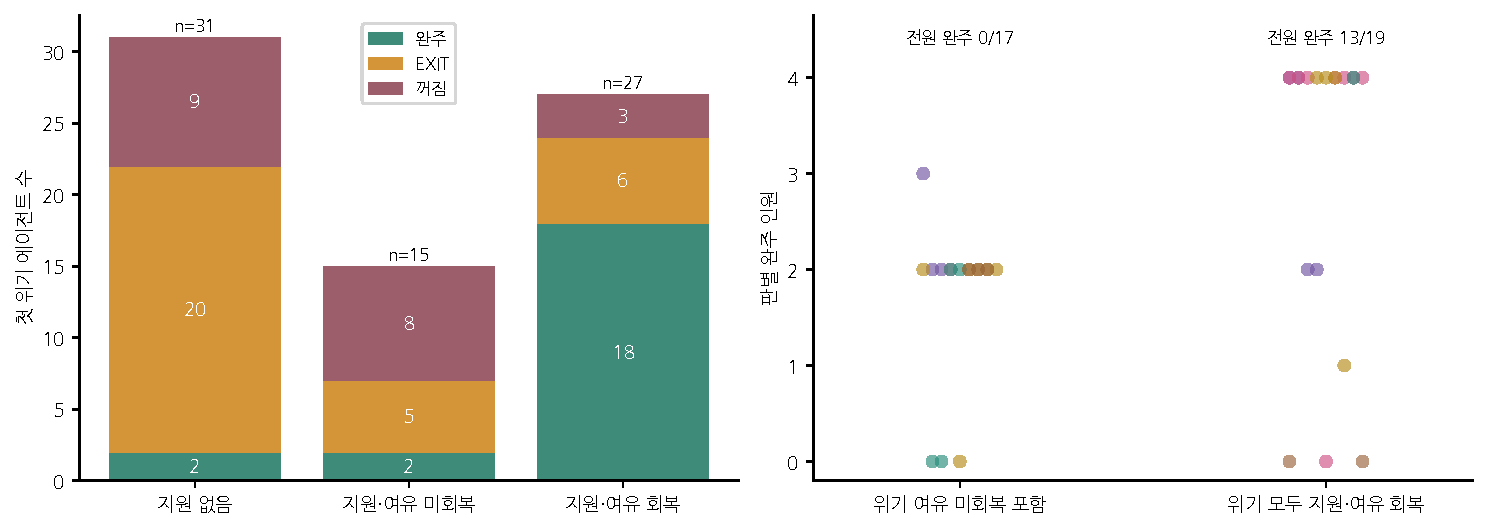
\includegraphics[width=\textwidth]{cogsci2027/ko/figures/appendix_refresh_20261107/crisis_followup_10games.pdf}
\caption{첫 위기 뒤 지원과 최종 완주. (a)는 오답 공개 뒤 대화 시작에 처음 $L<1$이 된 경우 중 8라운드 이전이고 다른 에이전트가 실제로 함께 있던 73명(43판)의 끝 상태다. 위기 라운드에 꺼진 경우도 포함한다. 지원 뒤 여유는 결과 뒤 대화 종료 시점의 잔액에서 확정 벌금을 차감했다. (b)는 각 판의 가장 이른 적격 첫 위기 시점에 네 명이 모두 있던 36판의 완주 인원이다. 당시 위기 에이전트가 모두 지원받고 대화 종료 시점에 $L\geq1$인 판과 그렇지 않은 판을 나누었다. 전원 완주는 각각 13/19판과 0/17판이다.}
\label{fig:appendix0-crisis-followup}
\end{figure}



\begin{figure}[H]
\centering
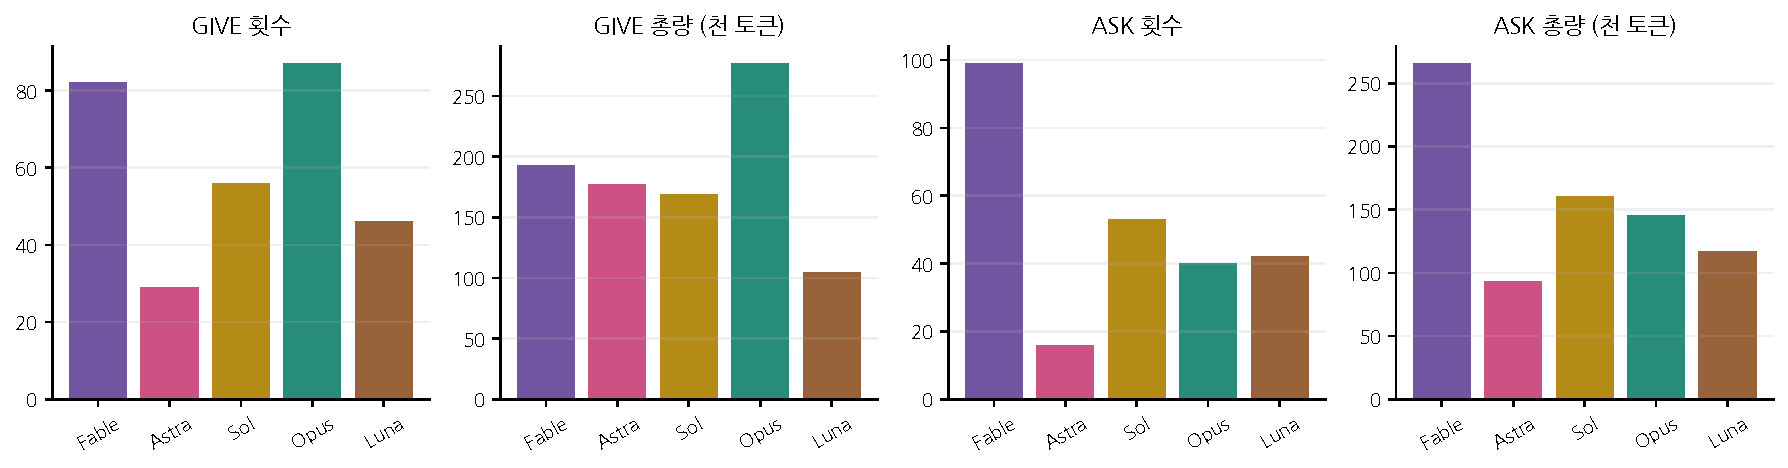
\includegraphics[width=\textwidth]{cogsci2027/ko/figures/appendix_refresh_20261107/give_ask_10games.pdf}
\caption{모델별 10판의 GIVE와 ASK 횟수 및 총량. 전체 50판에서 GIVE는 300건, ASK는 250건이다. 횟수는 성사된 행동 사건 수로 같은 응답의 여러 행동도 각각 센다. GIVE에는 재이전이, ASK에는 반복 요청이 포함된다. ASK 성사는 요청 발행을 뜻한다. 총량은 천 토큰 단위다.}
\label{fig:appendix0-give-ask}
\end{figure}
